\begin{fullwidth}
\chapter{Circuit Quantum Electrodynamics}\label{chap:cQED}
\end{fullwidth}
While many quantum mechanical systems can be used to create a qubit system, the focus of this thesis will be to treat quantum systems made on chips using superconducting materials. An overview of, how these qubits are formed and altered will be covered in this chapter.\\

\section{Circuit QED}
The basis is superconducting qubits is to use electronic circuits to form our potential. Usually, circuits would exhibit loss and follow the laws of classical electrodynamics, but by creating the devices from superconducting materials and cooling them down to $\approx 20 \unit{mK}$, the system will not dissipate energy. Thus they can be used as a platform for a qubit system.

Classically\, we define the dynamics of a circuit in terms of its current $I(t)$ and its voltage drop $V(t)$. Now to write up the Lagrangian in flux/charge basis which are conjugated variables. Using flux basis we define:
\begin{equation}
    \Phi (t) = \int_{-\infty}^t V(t')dt'
\end{equation}
Now using this relations together with $V = L dI/dt$ and $I = C dV/dt$ it is possible to find the energy by:
\marginnote[0.5 cm]{The lower integration limit comes from the assumption that the system was at rest at infinity}
\begin{equation}\label{eq: Energy from current and voltage}
    E(t) = \int_{-\infty}^t V(t')I(t')dt'
\end{equation}
Such that the energy of the components are:
\begin{equation}
    E_{capacitor} = \frac12 C \dot{\Phi}^2; \quad E_{inductor} = \frac{1}{2L} \Phi^2
\end{equation}
Defining the capacitant energy as the kinetic energy $T_C$ and inductive energy as $U_L$, we can write the Lagrangian as:
\begin{equation}
    \mathcal{L} = T_C - U_L = \frac12 C \dot{\Phi}^2 - \frac{1}{2L} \Phi^2
\end{equation}
And from this the Hamiltonian:\footnote{By defining a canonical momentum $Q = \partial \mathcal{L} / \partial \dot{\Phi}$ and doing the legendre transformation $\mathcal{H} = Q\dot{\Phi} - \mathcal{L}$.} \cite{krantz_quantum_2019}:
\begin{equation}
    \mathcal{H} = \frac{1}{2C} Q^2 + \frac{1}{2L} \Phi^2
\end{equation}

\subsection{Going quantum}
$\Phi$ and $Q$ are classical, conjugate variables and satisfy the Poisson bracket:
\begin{equation}
    \{ \Phi, Q\} = \pfrac{\Phi}{\Phi}\pfrac{Q}{Q} - \pfrac{\Phi}{Q}\pfrac{Q}{\Phi} = 1
\end{equation}
To quantize these parameters, we replace the variables with the corresponding operators: $Q \to \hat{Q}$ and $\Phi \ \to \hat{\Phi}$. And using the correspondence principle to replace the Poisson brackets with the commutator $\{...\} \to i\hbar[...]$. We have \cite{krantz_quantum_2019}:
\begin{equation}
    [\hat{\Phi}, \hat{Q}] = i\hbar
\end{equation}



\section{Forming Qubits}\label{sec:forming_qubits}
As a start, we consider the LC-circuit which consist of a single capacitive element and one inducting. This exactly yields the Hamiltonian $\mathcal{H} = \mathcal{H} = \frac{1}{2C} Q^2 + \frac{1}{2L} \Phi^2$. When considering a flux basis, we need 
\begin{marginfigure}[1 cm]
    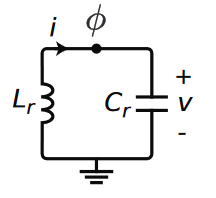
\includegraphics[width = \linewidth]{tex/fig_for_text/LC_circuit.png}
    \caption{Circuit diagram for the LC circuit.}
\end{marginfigure}
\begin{equation}
    \hat{Q} = i\hbar \pfrac{}{\hat{\Phi}}
\end{equation}
for the commutator relation to be satisfied. Dropping the hats and setting $\hbar = 1$
\begin{equation}
    H \ket{\psi} = - \frac{1}{2C} \pfracsquared{}{\Phi}\ket{\psi} + \frac{1}{2L} \Phi^2 \ket{\psi}
\end{equation}
Here we can follow the derivations from harmonic oscillators and define the ladder operators, $a, a^\dagger$. Such that the the Hamiltonian can be written as:
\begin{equation}
    H = \omega (a^\dagger a + \frac12)
\end{equation}
Where $\omega = \sqrt{8 E_C E_L}$ can be found by comparing the hamiltonian with the one from the harmonic oscillator.

While the harmonic oscillator has an abundance of nice properties for physics, it has equidistant energy levels. Driving oscillations with the frequency $\omega$ will not only contribute to transitions in the computational basis ($\ket{0}, \ket{1}$), but also all states $\ket{n}$ where $n > 1$. With this leakage quantum computing will be impossible, and for this reason, we must search for an anharmonic potential.

\subsection{The Josephson Junction}
The solution lies in another component, which is accessible in the superconducting circuit. By separating two superconductors by a semiconducting material, the Cooper pairs will no longer travel through without resistance but will instead have a probability of tunneling through the insulator/superconductor. This probability is dependent on the phase difference between the two superconductors. 
\marginnote[0.5 cm]{Probably an idea to derive the Josephson junction, maybe just for my own sake.}

The probability for tunneling through the superconducting phase is given as $\sin[2e\phi(t) / \hbar]$, where $\phi(t)$ is the time-dependent difference in phase between the two superconductors which are separated by the junction. Using the flux-quantum $\phi_0 = h / 2e$ and adding an external flux, the current through the Josephson Junction is:
\begin{equation}
    I(t) = I_0 \sin \left[ \frac{\phi(t) + \phi_{ext}}{\phi_0} \right]
\end{equation}
Which can be integrated according to equation \ref{eq: Energy from current and voltage} to get an energy:
\begin{equation}
    E_{\text{Josephson Junction}} = - E_J \cos \left[ \frac{\phi(t) + \phi_{ext}}{\phi_0} \right]
\end{equation}
up to a constant, which can be neglected by setting the zero point of the energy. \cite{vool_introduction_2017}

\subsection{The Cooper Pair Island}
Replacing the inductor with a Josephson Junction. We can instead obtain a circuit with a non-quadratic energy term. The hamitlnoian is given by:
\begin{marginfigure}
    \caption{An example of a circuit with a capacitor and a Josephson Junction}
    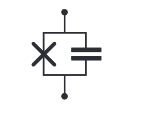
\includegraphics[width = \textwidth]{tex/fig_for_text/CooperPairIsland.png}
    \label{fig:cooper_pair_island}
\end{marginfigure}

\begin{equation}
    H(t) =  4 E_C (n - n_g)^2 -  E_J \cos \left[ \frac{\phi(t) + \phi_{ext}}{\phi_0} \right]
\end{equation}

When we think of the charge to be similar to the kinetic energy and the flux part to give some sort of potential, illustrating the energy levels become easier. The potential and the few  and is typically done in the plots seen in fig. \ref{fig:cooper_pair_box_energy_levels}. The important part is to see, that the energy $E_2-E_1 \neq E_1 - E_0$, because of the introduced non-linearity from the Josephson Junction. The non-linearity is an important parameter for qubit control and also has gotten its own name, anharmonicity defined from the difference in frequencies (or energies if we reintroduce $\hbar$): $\alpha = \omega_{1, 2}- \omega_{0, 1}$. \todo{Cite original Cooper Pair Box Paper and check content} \cite{Bouchiat1}

\begin{figure}
    \centering
    \missingfigure{Cooper Pair Box - Energy levels}
    \caption{The flux-potential of the cooper pair box along with the three lowest energy levels. The anharmonicity is shown in relation to the energy differences between the three lowest levels.}
    \label{fig:cooper_pair_box_energy_levels}
\end{figure}

\subsection{The Transmon}
\todo{Take much more inspiration from the Koch article. At the moment it is just a draft with around the desired content.}
An important challenge of the Cooper Pair Island is the sensitivity to charge noise. While this can be canceled somewhat by being in a so-called "sweet spot", another chip design has been suggested. The Transmon is by many called the workhorse of superconducting qubits and this is not without reason. 

The Transmon deviates from the cooper pair box by an increased $E_J/E_C$ ratio of $\approx 30-100$ reducing the susceptibility to charge noise significantly. This comes at the cost of some anharmonicity, but it can still be kept large enough to have sufficient control of the qubits.\cite{koch_charge_2007}

\begin{figure*}
    \centering
    \missingfigure{Overview over the Transmon and its energy levels}
    \caption{Overview over the Transmon and its energy levels}
    \label{fig:transmon_energy_levels}
\end{figure*}

Further variations of the Transmon provide tuneability of the qubit frequency by either implementing a squid-loop where the flux through it alters the energy or by using a nano-wire design 



\section{Numerical cQED}
In an attempt to simulate the systems considered in this thesis, we will in this section introduce how the problems at hand is represented in a suitable way for solving numerically. As mentioned in the previous sections, the Hamiltonian is made out of the two conjugate operators $\hat{\phi}$ and $\hat{n}$ satisfying the commutation relation $\comm{\hat{\phi}}{\hat{n}} = i\hbar$. Like position and momentum, we now have a choice of which basis to represent the system in. In mechanical quantum problem, we would for example consider the position basis $\hat{x}$ and the canonical momentum would now become $\hat{p} = i \hbar \pfrac{}{\hat{x}}$. \cite{aumann_circuitq_2022}
\todo{Do we need a superconducting section that leads up to this section? }

The two basis are related to each other by the Fourier-like transformation \cite{langford} \footnote{This is very similar to the relation between $x$ and $p$, but with the extra detail that $n$ is discrete and $\phi\in[0, 2\pi]$.}:
\begin{align}
    \ket{\phi} &= \sum_{n=-\infty}^\infty e^{in\phi}\ket{N} \\
    \ket{n} &= \frac{1}{2\pi} \int_0^{2\pi}d\phi e^{-in\phi}\ket{\phi}
\end{align}

giving us the possibility to change basis on demand. Often the problem at hand will be easier to formulate in one basis rather than the other. For the transmon, the charge is often localized around 0 and it will be easier to set a limit on the $n_{\text{cutoff}}$ making it a good choice. 

In the charge basis, the energy associated with $\hat{q} = 2e\hat{n}$ takes a diagonal form. When restricted us to a finite value of $n_{\text{cutoff}}$ the charge (or number operator) takes the form\footnote{Since most of the qubit scale with a term $E_C(\hat{n} - n_g)^2$ we will only consider the lower energy states, which will be the goal in the end anyways.}:

\begin{equation}
    \hat{q} =  2 e \hat{n} = 2 e \begin{bmatrix}
-n_{\text{cutoff}} & 0 &  & \ldots &  \\
0 & -n_{\text{cutoff}}+1 &  &  &  \\
 &  & \ddots &  &  \\
\vdots &  &  & n_{\text{cutoff}}-1 &  \\
 &  &  &  & n_{\text{cutoff}} 
\end{bmatrix}
\end{equation} 

To represent the $\cos(\hat{\phi} / \phi_0)$ in the charge basis, we will use that:
\begin{align*}
    e^{\pm i \hat{\phi}}\ket{n} &= \frac{1}{2\pi} \int_0^{2\pi} d \phi' e^{-in\phi'} e^{\pm i \hat{\phi}}\ket{\phi'} \\
                                &=  \frac{1}{2\pi} \int_0^{2\pi} d \phi' e^{-in\phi'\pm i \phi'} \ket{\phi'} \\
                                &=  \frac{1}{2\pi} \int_0^{2\pi} d \phi' e^{-i\phi'(n\pm 1)} \ket{\phi'} = \ket{n\mp 1}\\                                
\end{align*}
Since this is true for all number states that the $e^{i\hat{\phi}}$ takes a state $\ket{n}$ and return $\ket{n+1}$, we can write it alternatively as:
\begin{equation}
    e^{i\hat{\phi}} = \sum_n = \ket{n}\bra{n+1}; \quad e^{-i\hat{\phi}} = \sum_n = \ket{n}\bra{n-1}
\end{equation}

Now decomposing the cosine into the complex exponentials, we can write this as:
\begin{fullwidth}
\begin{align}
    \cos(\hat{\phi}/\phi_0 + \phi_{ext}) &= \frac12 \left(e^{-i(\hat{\phi}/\phi_0 + \phi_{ext})} + e^{i(\hat{\phi}/\phi_0 + \phi_{ext}}))\right) \\
    &= \frac12 \left(e^{i\phi_{ext}}e^{i\hat{\phi}/\phi_0} + e^{-i\phi_{ext}}e^{-i\hat{\phi}/\phi_0}\right)  \\
    &= \frac12 \sum_n \left(e^{i\phi_{ext}} \ket{n}\bra{n + 1} + e^{-i\phi_{ext}} \ket{n}\bra{n+ 1}   \right) \\
    &= \frac12 \begin{pmatrix}
        0 & e^{-i\phi_{ext}} & 0 & \hdots \\
        e^{i\phi_{ext}} & 0 & e^{-i\phi_{ext}} \\
        0 & e^{i\phi_{ext}} & 0 & \\
        \vdots & & & \ddots 
    \end{pmatrix}
\end{align}
\end{fullwidth}
With the reprensentation of the charge $q = 2e\hat{n}$ and the $\cos{\hat{\phi}}$, we are now in a position to write up the Hamiltonian of a Cooper Pair Box or a Transmon in a discretized matrix. Of course we could expand this formalism to other operators or go the flux basis if we were to consider other devices like Fluxonium or sometging more elaborate.
\todo{Check the details here like which is a plus and which is a minus. n, n+1 and that kind of stuff.}
In simplest version with $\phi_{ext} = 0$ this all just becomes a matrix with two off-diagonal of 1. 

\todo{Write in the flux-basis. Will be short when the general introduction is made}

With a discrete matrix representation of the charge matrix and flux operators, we are in a position to calculate the eigen-energies and states of a given Hamiltonian. This is done by numerically determening the eigenvalues/vectors of the hamiltonian matrix. In figure \ref{fig:transmon_numerically_solved} the transmon is solved and the energy levels is shown in the flux- basis and charge basis along with the wave functions of the qubit states. By limiting us to the few lowest energy eigenstates because of the low temperature, we can reduce the basis significantly to the energy representation, where the Hamiltonian is diagonal: $H = \sum_k^{k_{max}} \hbar \omega_k \ket{k}\bra{k}$ where $k$ refers to the k'th lowest energy eigenvalue of the Hamiltonian.

\begin{figure}
    \centering
    \missingfigure{A demonstration of the eigenstates of the Transmon along with its eigenstates.}
    \caption{Caption}
    \label{fig:transmon_numerically_solved}
\end{figure}



% \textbf{Rambling now. Tighten the following: from . The part with }

% When considering the circuits like the transmon with $\frac{E_C}{E_J}\approx 50$ the dominating term in the hamiltnonian will be the contribution from the charge offset proportional to $(\hat{n} - n_g)^2$. This is a good indication that the charge matrix would be good choice to contain as much information as possible near the diagonal. In the charge basis the charge matrix simply takes the form:

% where $n_{\text{cutoff}}$ is an appropriately set parameter to limit the size of our hilbert space. With the parameters used, this is normally set around 50-100. \\

% With the choice of $n$ as eigenbasis the operator representation for flux will be $\hat{\phi} = \pfrac{}{\hat{n}}$ in the continuous basis or for finite dimensional Hilbert space, we have:
% \begin{equation}
%     \hat{\phi} = 
% \end{equation}

% \textbf{Probably do the transmon in the flux basis? }





% \vspace{2 cm}
% \textbf{This could also be a numerical section between section 2.1 and 2.2 which we can base the cooper pair box on. }
% When using the transmon, we use the energy eigenstates as a computational basis. To figure out, how the energy splitting and reactions to charge are, we need to find these energy eigenenergies and states.

% \begin{itemize}
%     \item Start with charge basis
%     \item We can now represent the flux as a potential
%     \item Solving numerically gives lowest eigenenergy and states
%     \item Calculating certain matrix elements between the eigenstates givers us the charge-matrix, flux-matrix, etc.. 
% \end{itemize}


\section{Experimental Setup}
I should have this... Is this the right place? 

\subsection{Cooling}

\subsection{Amplication}

\subsection{Specs}








